% Latex header for doxygen 1.8.9.1
\documentclass[twoside]{book}

% Packages required by doxygen
\usepackage{fixltx2e}
\usepackage{calc}
\usepackage{doxygen}
\usepackage[export]{adjustbox} % also loads graphicx
\usepackage{graphicx}
\usepackage[utf8]{inputenc}
\usepackage{makeidx}
\usepackage{multicol}
\usepackage{multirow}
\PassOptionsToPackage{warn}{textcomp}
\usepackage{textcomp}
\usepackage[nointegrals]{wasysym}
\usepackage[table]{xcolor}

% Font selection
\usepackage[T1]{fontenc}
\usepackage[scaled=.90]{helvet}
\usepackage{courier}
\usepackage{amssymb}
\usepackage{sectsty}
\renewcommand{\familydefault}{\sfdefault}
\allsectionsfont{%
  \fontseries{bc}\selectfont%
  \color{darkgray}%
}
\renewcommand{\DoxyLabelFont}{%
  \fontseries{bc}\selectfont%
  \color{darkgray}%
}
\newcommand{\+}{\discretionary{\mbox{\scriptsize$\hookleftarrow$}}{}{}}

% Page & text layout
\usepackage{geometry}
\geometry{%
  a4paper,%
  top=2.5cm,%
  bottom=2.5cm,%
  left=2.5cm,%
  right=2.5cm%
}
\usepackage[T1]{fontenc}
\usepackage{titlesec, blindtext, color}
\definecolor{gray75}{gray}{0.75}
\newcommand{\hsp}{\hspace{20pt}}
\titleformat{\chapter}[hang]{\Huge\bfseries}{\thechapter\hsp\textcolor{gray75}{|}\hsp}{0pt}{\Huge\bfseries}
\tolerance=750
\hfuzz=15pt
\hbadness=750
\setlength{\emergencystretch}{15pt}
\setlength{\parindent}{0cm}
\setlength{\parskip}{0.2cm}
\makeatletter
\renewcommand{\paragraph}{%
  \@startsection{paragraph}{4}{0ex}{-1.0ex}{1.0ex}{%
    \normalfont\normalsize\bfseries\SS@parafont%
  }%
}
\renewcommand{\subparagraph}{%
  \@startsection{subparagraph}{5}{0ex}{-1.0ex}{1.0ex}{%
    \normalfont\normalsize\bfseries\SS@subparafont%
  }%
}
\makeatother

% Headers & footers
\usepackage{fancyhdr}
\pagestyle{fancyplain}
\fancyhead[LE]{\fancyplain{}{\bfseries\thepage}}
\fancyhead[CE]{\fancyplain{}{}}
\fancyhead[RE]{\fancyplain{}{\bfseries\leftmark}}
\fancyhead[LO]{\fancyplain{}{\bfseries\rightmark}}
\fancyhead[CO]{\fancyplain{}{}}
\fancyhead[RO]{\fancyplain{}{\bfseries\thepage}}
\fancyfoot[LE]{\fancyplain{}{}}
\fancyfoot[CE]{\fancyplain{}{}}
\fancyfoot[RE]{\fancyplain{}{\bfseries\scriptsize Generated by Yu Chen }}
\fancyfoot[LO]{\fancyplain{}{\bfseries\scriptsize Generated by Yu Chen }}
\fancyfoot[CO]{\fancyplain{}{}}
\fancyfoot[RO]{\fancyplain{}{}}
\renewcommand{\footrulewidth}{0.4pt}
\renewcommand{\chaptermark}[1]{%
  \markboth{#1}{}%
}
\renewcommand{\sectionmark}[1]{%
  \markright{\thesection\ #1}%
}

% Indices & bibliography
\usepackage{natbib}
\usepackage[titles]{tocloft}
\setcounter{tocdepth}{3}
\setcounter{secnumdepth}{5}
\makeindex

% Hyperlinks (required, but should be loaded last)
\usepackage{ifpdf}
\ifpdf
  \usepackage[pdftex,pagebackref=true]{hyperref}
\else
  \usepackage[ps2pdf,pagebackref=true]{hyperref}
\fi
\hypersetup{%
  colorlinks=true,%
  linkcolor=blue,%
  citecolor=blue,%
  unicode%
}

% Custom commands
\newcommand{\clearemptydoublepage}{%
  \newpage{\pagestyle{empty}\cleardoublepage}%
}


%===== C O N T E N T S =====

\usepackage[yyyymmdd,hhmmss]{datetime}

\begin{document}

% Titlepage & ToC
\hypersetup{pageanchor=false,
             bookmarks=true,
             bookmarksnumbered=true,
             pdfencoding=unicode
            }
\pagenumbering{roman}
\begin{titlepage}
\vspace*{7cm}
\begin{center}%
{\Huge Dual State Framework}\\
\vspace*{0.5cm}
{\Large Research Documentation}\\
\vspace*{1cm}
{\normalsize Yu Chen - C00151352}\\
\vspace*{0.2cm}
{\small \today\ \currenttime}\\
\end{center}
\end{titlepage}
\clearemptydoublepage
\chapter*{Abstract}
\label{_abstract}
\hypertarget{_abstract}{}
This report was commissioned to investigate the possibility of developing the library Dual State Framework that helps programmers implement parallel computing easily. The research covers\+:
\begin{DoxyItemize}
\item programming languages
\item libraries for Graphics
\item libraries of parallel programming
\item integrated development environments
\item source control tools
\item documentation tools
\item software packaging tools
\end{DoxyItemize}

According to the investigation, I think it is not hard to complete the project. The correct combination of Open Source and free applications seems to be the best choice to develop the framework.
\begin{DoxyItemize}
\item C++
\item S\+F\+M\+L
\item Intel T\+B\+B
\item Xcode
\item Git
\item Doxygen, Graphviz, and La\+Tex
\item Package\+Maker, Installforge, Debreate 
\end{DoxyItemize}
\tableofcontents
\clearemptydoublepage
\pagenumbering{arabic}
\hypersetup{pageanchor=true}

%--- Begin generated contents ---
\chapter{Overview}
\label{_overview}
\hypertarget{_overview}{}
\hypertarget{_overview_LockerinThreadSafety}{}\section{Locker in Thread Safety}\label{_overview_LockerinThreadSafety}
In the context of multi-\/threaded programs, shared data and be read and written by multiple threads during simultaneous execution. To keep the data correct, usually a locker is required. The function of locker is to make data to be accessed by only one thread at any given time. For example, one thread tries to update the data. It locks the data to make it inaccessible by any other threads. After change, it can unlock the data and now the data is available for all threads. The disadvantage of locker is if one thread need to access the data but the data is locked by another thread, it should wait until the data is unlocked. ~\newline
~\newline
\label{_overview_eg1}%
\hypertarget{_overview_eg1}{}%
Example 1 
\begin{DoxyImageNoCaption}
  \mbox{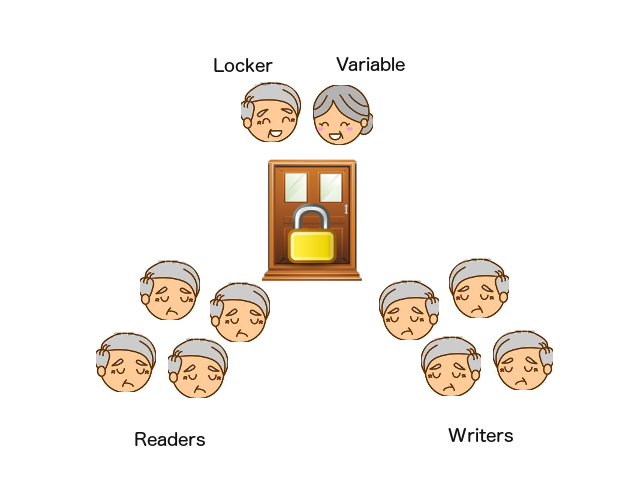
\includegraphics[width=\textwidth,height=\textheight/2,keepaspectratio=true]{ResearchOverviewLockerinThreadSafety.png}}
\end{DoxyImageNoCaption}

\begin{DoxyItemize}
\item A variable is locked by a thread
\item 100 threads need to read the variable
\item 100 threads need to write the variable
\end{DoxyItemize}

In this case, 200 threads are waiting for one variable.\hypertarget{_overview_Theideaofthisproject}{}\section{The idea of this project}\label{_overview_Theideaofthisproject}
The idea of this project is to make the variable in to two states\+: one for read and the other one for write. This is why the project name is Dual State Framework. Any time, a thread tries to lock the variable will lock the write copy. The read copy is always available for all thread. It means only threads that try to write the variable need wait. Back to \hyperlink{_overview_eg1}{Example 1}, now we have only 100 threads are waiting. 
\begin{DoxyImageNoCaption}
  \mbox{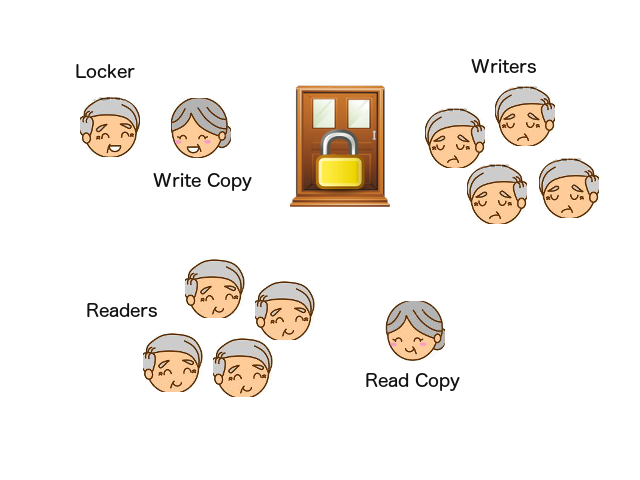
\includegraphics[width=\textwidth,height=\textheight/2,keepaspectratio=true]{ResearchOverviewTheideaofthisproject.png}}
\end{DoxyImageNoCaption}
 
\chapter{Game Development}
\label{_game_development}
\hypertarget{_game_development}{}
Games development is one of the most exciting areas of software development that you can work in. Game developers require skills and expertise in modeling, graphics programming, game design, simulation and animation.\hypertarget{_game_development_GameDevelopmentGraphicsAPIs}{}\section{Graphics A\+P\+Is}\label{_game_development_GameDevelopmentGraphicsAPIs}
\hypertarget{_game_development_GameDevelopmentGraphicsAPIsOpenGL}{}\subsection{Open\+G\+L}\label{_game_development_GameDevelopmentGraphicsAPIsOpenGL}
Open\+G\+L is a multi-\/platform A\+P\+I for developing 2\+D and 3\+D graphics applications. Most of Libraries is based on Open\+G\+L, such as S\+F\+M\+L. Open\+G\+L is the industry\textquotesingle{}s most widely used and supported 2\+D and 3\+D graphics application programming interface, bringing thousands of applications to a wide variety of computer platforms. \cite{opengl}\hypertarget{_game_development_GameDevelopmentGraphicsAPIsMicrosoftDirectX}{}\subsection{Microsoft Direct\+X}\label{_game_development_GameDevelopmentGraphicsAPIsMicrosoftDirectX}
Microsoft Direct\+X is a collection of A\+P\+Is designed to allow development of games and multimedia applications on Microsoft platforms. It is the graphics technology powering today’s most impressive games.\hypertarget{_game_development_GameDevelopmentGraphicsAPIsComparison}{}\subsection{Open\+G\+L vs. Direct\+X}\label{_game_development_GameDevelopmentGraphicsAPIsComparison}
\begin{TabularC}{3}
\hline
\rowcolor{lightgray}{\bf Feature\+: }&{\bf Open\+G\+L }&{\bf Direct\+X  }\\\cline{1-3}
Vertex Blending &N/\+A &Yes \\\cline{1-3}
Multiple Operating Systems &Yes &No \\\cline{1-3}
Extension Mechanism &Yes &Yes \\\cline{1-3}
Development &Multiple member Board &Microsoft \\\cline{1-3}
Thorough Specification &Yes &No \\\cline{1-3}
Two-\/sided lighting &Yes &No \\\cline{1-3}
Volume Textures &Yes &No \\\cline{1-3}
Hardware independent Z-\/buffers &Yes &No \\\cline{1-3}
Accumulation buffers &Yes &No \\\cline{1-3}
Full-\/screen Antialiasing &Yes &Yes \\\cline{1-3}
Motion Blur &Yes &Yes \\\cline{1-3}
Depth of field &Yes &Yes \\\cline{1-3}
Stereo Rendering &Yes &No \\\cline{1-3}
Point-\/size/line-\/width attributes &Yes &No \\\cline{1-3}
Picking &Yes &No \\\cline{1-3}
Parametric curves and surfaces &Yes &No \\\cline{1-3}
Cache geometry &Display Lists &Vertex Buffers \\\cline{1-3}
System emulation &Hardware not present &Let app determine \\\cline{1-3}
Interface &Procedure calls &C\+O\+M \\\cline{1-3}
Updates &Yearly &Yearly \\\cline{1-3}
Source Code &Sample &S\+D\+K Implementation \\\cline{1-3}
\end{TabularC}
\cite{openglvsd3x}\hypertarget{_game_development_GameDevelopmentMultimediaLibraries}{}\section{Multimedia Libraries}\label{_game_development_GameDevelopmentMultimediaLibraries}
\hypertarget{_game_development_GameDevelopmentMultimediaLibrariesSFML}{}\subsection{S\+F\+M\+L}\label{_game_development_GameDevelopmentMultimediaLibrariesSFML}
S\+F\+M\+L (Simple and Fast Multimedia Library) is a portable A\+P\+I written in C++ for multimedia programming based on Open\+G\+L and Open\+A\+L. It supports multiple programming languages such as C++ , Python, .Net and etc. It can be thought of as an object oriented alternative to S\+D\+L. S\+F\+M\+L provides hardware accelerated 2\+D graphics, and supports Open\+G\+L windowing and provides different modules that ease multimedia and game programming. \cite{sfml} \hypertarget{_game_development_GameDevelopmentMultimediaLibrariesSDL}{}\subsection{S\+D\+L}\label{_game_development_GameDevelopmentMultimediaLibrariesSDL}
S\+D\+L (Simple Direct\+Media Layer) is a cross-\/platform development library designed to provide low level access to hardware via Open\+G\+L and Direct3\+D. It support multiple programming languages (C/\+C++, python, .Net and etc.) \cite{sdl} 
\chapter{Parallel Programming Model}
\label{_parallel_programming_model}
\hypertarget{_parallel_programming_model}{}
Parallel programming model is a set of software technologies to express parallel algorithms and match applications with the underlying parallel systems. \hypertarget{_parallel_programming_model_ParallelProgrammingModelSerialComputingvsParallelComputing}{}\section{Serial Computing vs Parallel Computing}\label{_parallel_programming_model_ParallelProgrammingModelSerialComputingvsParallelComputing}
\begin{TabularC}{2}
\hline
\rowcolor{lightgray}{\bf Serial Computing }&{\bf Parallel Computing  }\\\cline{1-2}
A problem is broken into a discrete series of instructions &A problem is broken into discrete parts that can be solved concurrently \\\cline{1-2}
Instructions are executed sequentially one after another &Each part is further broken down to a series of instructions \\\cline{1-2}
Executed on a single processor &Instructions from each part execute simultaneously on different processors \\\cline{1-2}
Only one instruction may execute at any moment in time &An overall control/coordination mechanism is employed \\\cline{1-2}
\end{TabularC}
\hypertarget{_parallel_programming_model_ParallelProgrammingModelSerialComputingvsParallelComputingSerialComputingDiagram}{}\subsection{Serial Computing Diagram}\label{_parallel_programming_model_ParallelProgrammingModelSerialComputingvsParallelComputingSerialComputingDiagram}

\begin{DoxyImageNoCaption}
  \mbox{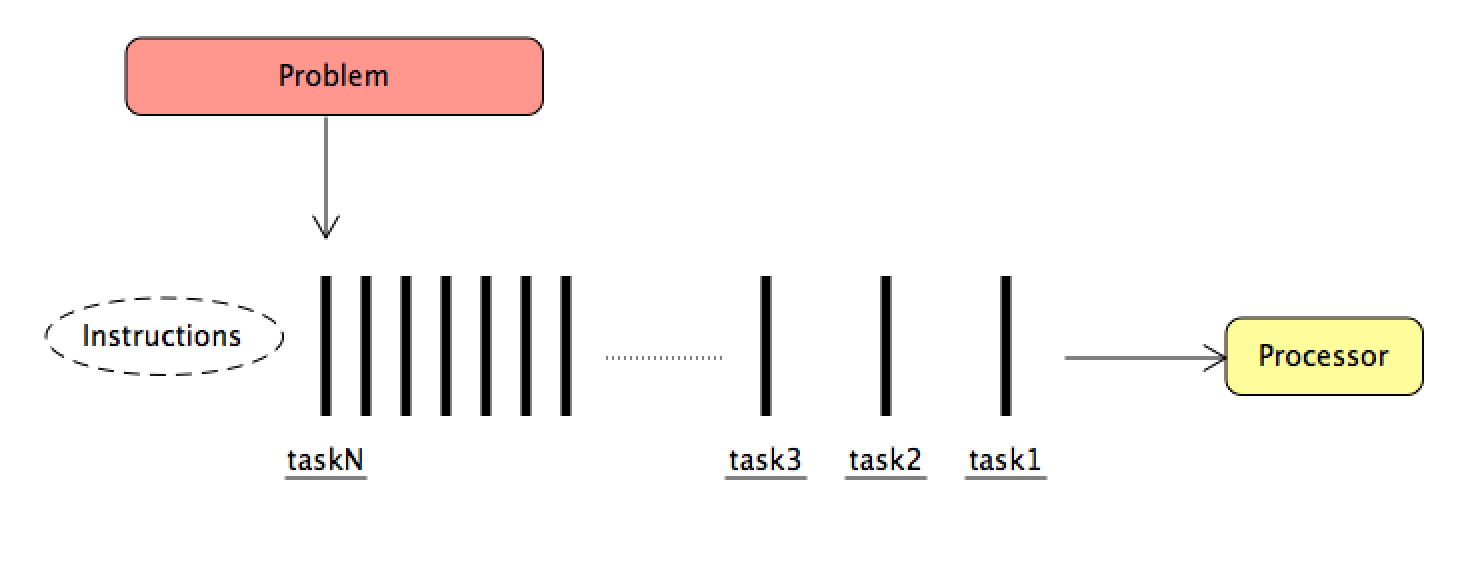
\includegraphics[width=\textwidth,height=\textheight/2,keepaspectratio=true]{ResearchSerialComputingDiagram.png}}
\end{DoxyImageNoCaption}
 \hypertarget{_parallel_programming_model_ParallelProgrammingModelSerialComputingvsParallelComputingParallelComputingDiagram}{}\subsection{Parallel Computing Diagram}\label{_parallel_programming_model_ParallelProgrammingModelSerialComputingvsParallelComputingParallelComputingDiagram}

\begin{DoxyImageNoCaption}
  \mbox{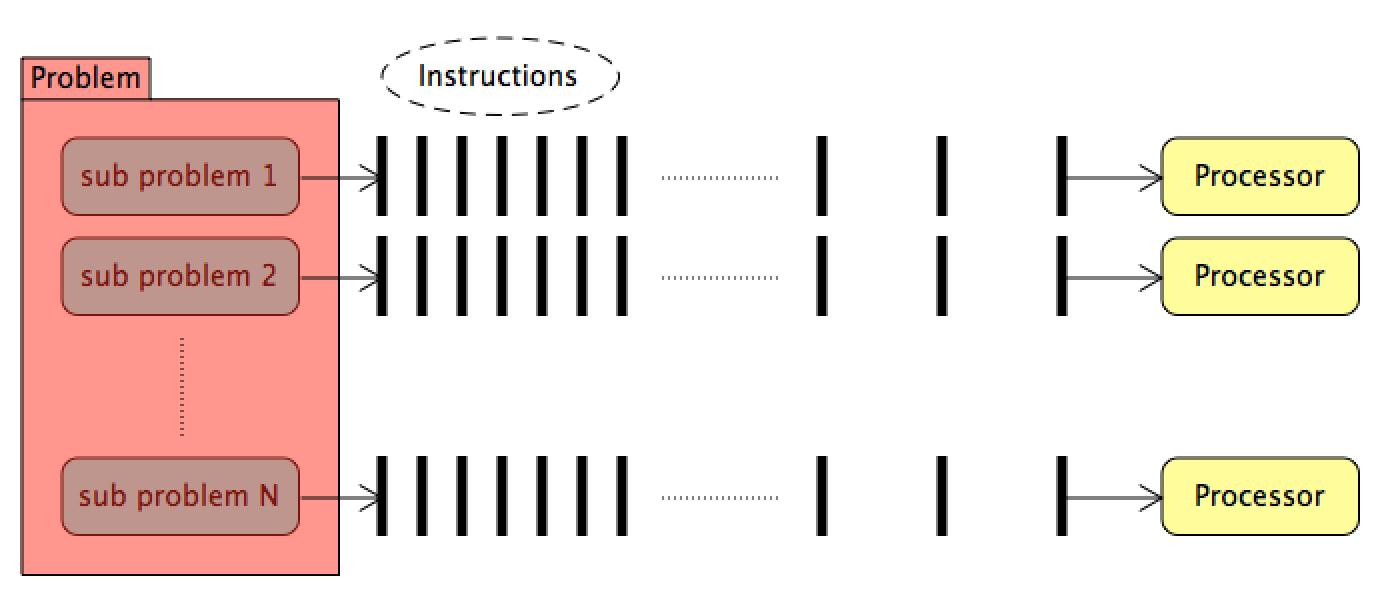
\includegraphics[width=\textwidth,height=\textheight/2,keepaspectratio=true]{ResearchParallelComputingDiagram.png}}
\end{DoxyImageNoCaption}
\hypertarget{_parallel_programming_model_ParallelProgrammingModelOpenMP}{}\section{Open\+M\+P}\label{_parallel_programming_model_ParallelProgrammingModelOpenMP}
The Open Multi-\/\+Processing (Open\+M\+P) is a library that can be used to specify shared memory parallelism in Fortran and C/\+C++ programs. It provides a model for parallel programming that is portable across shared memory architectures from different vendors. The benefit of Open\+M\+P is it is very easy. Open\+M\+P is compiler directive based that means to use Open\+M\+P you need a open\+M\+P supported Compiler.\+More information about the Open\+M\+P A\+P\+I can be found at \href{http://www.openmp.org}{\tt http\+://www.\+openmp.\+org}.\hypertarget{_parallel_programming_model_ParallelProgrammingModelIntelTBB}{}\section{Intel T\+B\+B}\label{_parallel_programming_model_ParallelProgrammingModelIntelTBB}
Intel Threading Building Blocks (Intel T\+B\+B) is a C and C++ library for creating high performance and scalable parallel applications. It provides a set of interfaces, functions, and renders for implementing parallelism. The advantage of Intel T\+B\+B is it is not compiler directive based as Open\+M\+P that means you can use whatever compiler you preferred.\hypertarget{_parallel_programming_model_ParallelProgrammingModelConcurrencyModel}{}\section{Concurrency Model}\label{_parallel_programming_model_ParallelProgrammingModelConcurrencyModel}
Concurrency is a property of systems in which several computations are executing simultaneously, and potentially interacting with each other. ~\newline
~\newline
Concurrency vs Parallelism \cite{parallelismVsConcurrency} \begin{TabularC}{2}
\hline
\rowcolor{lightgray}{\bf Concurrency }&{\bf Parallelism  }\\\cline{1-2}
Concurrency is when two tasks can start, run, and complete in overlapping time periods. It doesn\textquotesingle{}t necessarily mean they\textquotesingle{}ll ever both be running at the same instant. Eg. multitasking on a single-\/core machine. &Parallelism is when tasks literally run at the same time. Eg. on a multicore processor. \\\cline{1-2}
Eg. multitasking on a single-\/core machine. &Eg. on a multicore processor. \\\cline{1-2}
A condition that exists when at least two threads are making progress. A more generalized form of parallelism that can include time-\/slicing as a form of virtual parallelism. &A condition that arises when at least two threads are executing simultaneously. \\\cline{1-2}
\end{TabularC}
~\newline
~\newline
Example Concurrency Models\+:
\begin{DoxyItemize}
\item Actors Model
\item C\+S\+P (Communicating Sequential Processes)
\item Disruptor
\item Thread 
\end{DoxyItemize}
\chapter{Development Tools}
\label{_development_tools}
\hypertarget{_development_tools}{}
\hypertarget{_development_tools_DevelopmentToolsCppIDEsforMacOSX}{}\section{C++ I\+D\+Es for Mac O\+S X}\label{_development_tools_DevelopmentToolsCppIDEsforMacOSX}
\hypertarget{_development_tools_DevelopmentToolsCppIDEsforMacOSXXcode}{}\subsection{Xcode}\label{_development_tools_DevelopmentToolsCppIDEsforMacOSXXcode}
Xcode is the default software development I\+D\+E for Mac os X. It provides everything developers need to create great applications for Apple computers (Mac, i\+Phone, and i\+Pad). Xcode has a good interface design, a good start up speed, and a good tool set for debugging. \hypertarget{_development_tools_DevelopmentToolsCppIDEsforMacOSXNetBeans}{}\subsection{Net\+Beans}\label{_development_tools_DevelopmentToolsCppIDEsforMacOSXNetBeans}
Net\+Beans I\+D\+E is originally built for Java development. It has a good scalability that provides plugins for C++ development. It is free and open source and has a large community of users and developers around the world. Net\+Beans is written in Java so that it may be slower compared to native binary applications. \hypertarget{_development_tools_DevelopmentToolsCppIDEsforMacOSXEclipse}{}\subsection{Eclipse}\label{_development_tools_DevelopmentToolsCppIDEsforMacOSXEclipse}
Eclipses is similar to Net\+Beans. The only difference may be it has more plugins and slower.\hypertarget{_development_tools_DevelopmentToolsDocumentation}{}\section{Documentation}\label{_development_tools_DevelopmentToolsDocumentation}
\hypertarget{_development_tools_DevelopmentToolsDocumentationDoxygen}{}\subsection{Doxygen}\label{_development_tools_DevelopmentToolsDocumentationDoxygen}
Doxygen is the documentation tool for generating A\+P\+I documentation from source code.\+It is developed under Mac os and Linux, but also it supports Window or other Unix-\/like operating systems. Doxygen supports languages like C++, C\#, Java, python, and etc. \hypertarget{_development_tools_DevelopmentToolsDocumentationGraphviz}{}\subsection{Graphviz}\label{_development_tools_DevelopmentToolsDocumentationGraphviz}
Graphviz is an open source graph visualization tool. It is easy to represent structural information as diagrams of abstract graphs and networks. Combining Doxygen and Graphviz can easily create O\+O\+P based U\+M\+L diagram. \hypertarget{_development_tools_DevelopmentToolsDocumentationUMLet}{}\subsection{U\+M\+Let}\label{_development_tools_DevelopmentToolsDocumentationUMLet}
U\+M\+Let is an open source U\+M\+L tool with a simple user interface. By using U\+M\+Let you can draw U\+M\+L diagrams very fast. It allows you build sequence and activity diagrams from plain text. U\+M\+Let is developped by Jave, so is runs on Windows, Mac O\+S X, Linux, and any Java supported device. An Eclipse plug-\/in is also available online. \hypertarget{_development_tools_DevelopmentToolsDocumentationLaTex}{}\subsection{La\+Tex}\label{_development_tools_DevelopmentToolsDocumentationLaTex}
La\+Te\+X is a high-\/quality typesetting system for the production of technical and scientific documentation. La\+Te\+X is not the name of a particular editing application. It refers to the encoding or tagging conventions that are used in La\+Te\+X documents. La\+Te\+X can be used as a standalone document preparation system, or as an intermediate format. La\+Te\+X is widely used in academia. \cite{latex} 
\chapter{Software Packaging}
\label{_software_packaging}
\hypertarget{_software_packaging}{}
Software packaging is the process used to put a software product into an installation package so that it can be installed by the users of the product on their computers. \hypertarget{_software_packaging_SoftwarePackagingOSXPackages}{}\section{O\+S X Packages}\label{_software_packaging_SoftwarePackagingOSXPackages}
In Mac O\+S X world, the installer packages have the file extension .pkg. Instead of distributing multiple files for a package, this allowed all of the software files to be contained in a single file for easier distribution with the benefit of package signing. Package\+Maker is part of the Xcode developer software suite. It provides a comfortable graphical user interface to help users create pkg installer easily. \cite{PackageMaker} 
\begin{DoxyImageNoCaption}
  \mbox{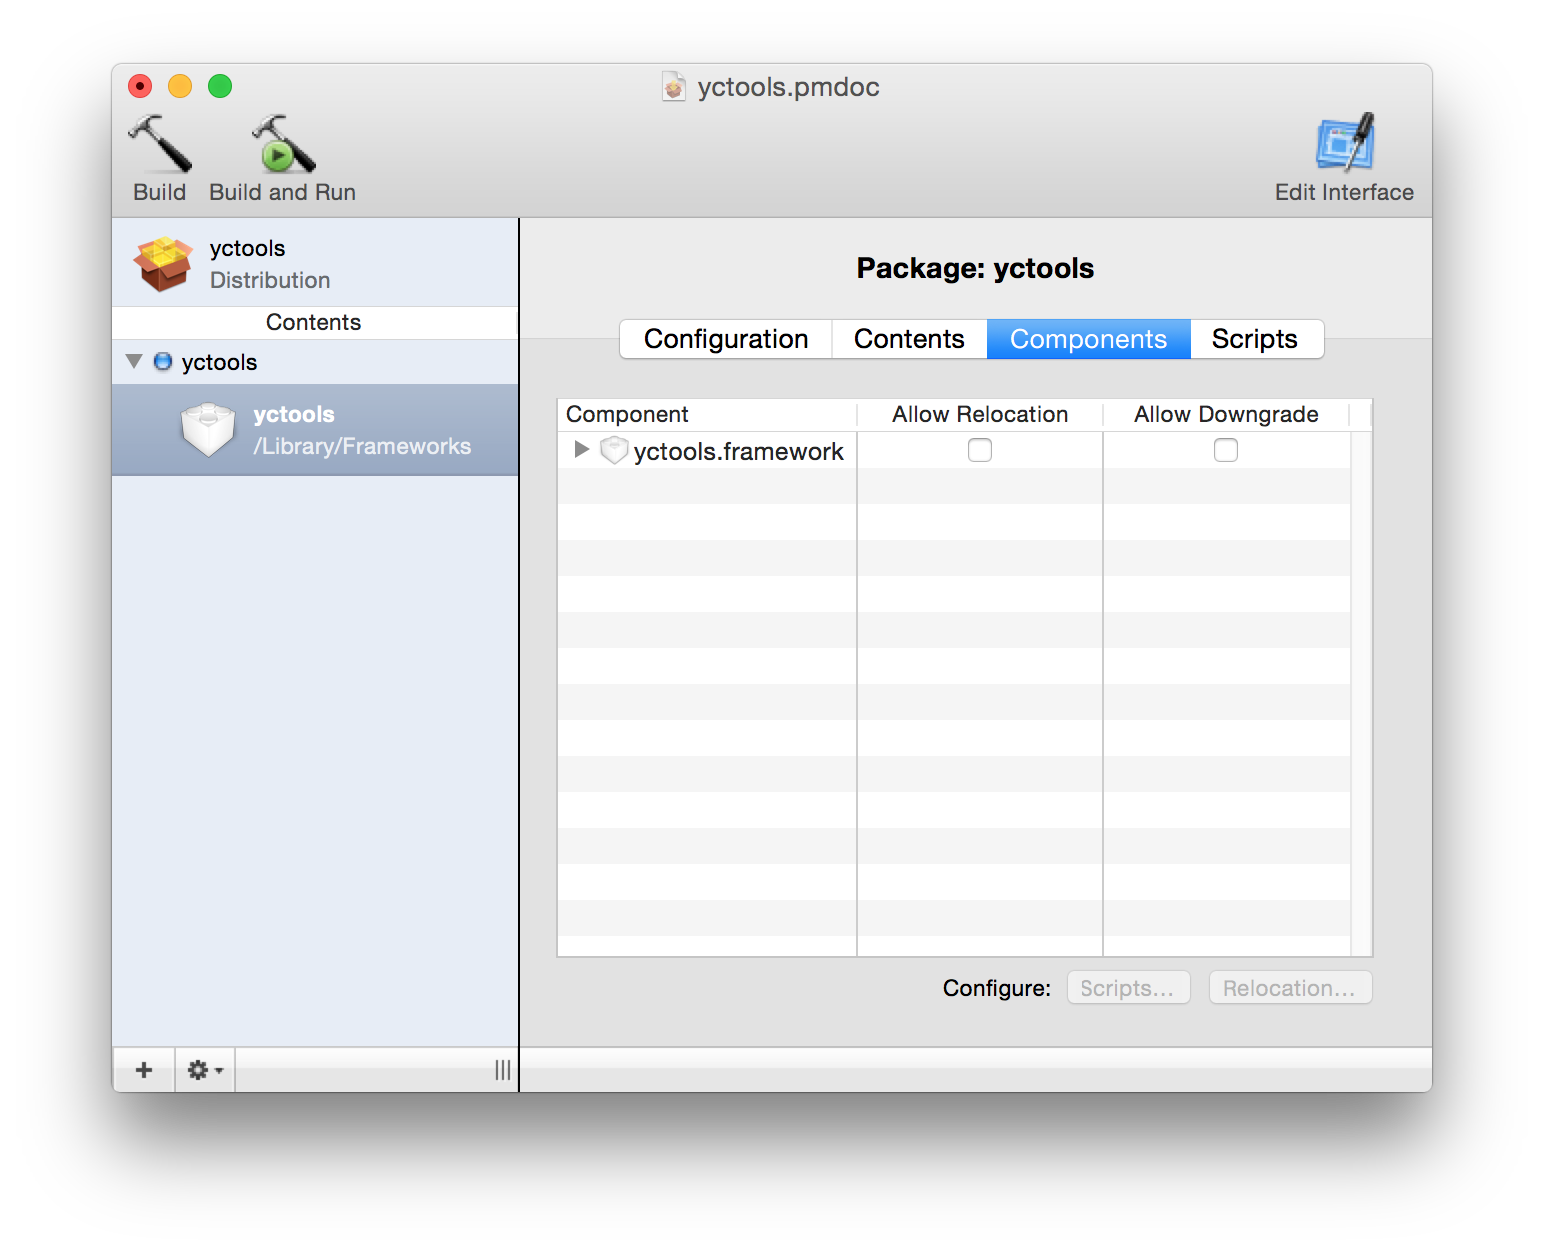
\includegraphics[width=\textwidth,height=\textheight/2,keepaspectratio=true]{ResearchPackegeMaker.png}}
\end{DoxyImageNoCaption}
\hypertarget{_software_packaging_SoftwarePackagingOSXBundle}{}\section{O\+S X Bundle}\label{_software_packaging_SoftwarePackagingOSXBundle}
A Mac O\+S X bundle is a directory that allows related resources such as executable files, graphics, and database to be grouped together, and appears as a single file to the user.
\begin{DoxyItemize}
\item A bundle with extension .app is an application bundle.
\item A framework is an bundle with extension .framework. It contains dynamic library files and header files.
\end{DoxyItemize}\hypertarget{_software_packaging_SoftwarePackagingWindowsInstaller}{}\section{Windows Installer}\label{_software_packaging_SoftwarePackagingWindowsInstaller}
The Windows Installer is a software component used for the software packaging in Windows world. The component contains installation, maintenance, and removal of software. ~\newline
~\newline
Install\+Forge is a free installation creator. It provides a series of functions such as interface design, system environment variable settings, and software update. \cite{installforge} 
\begin{DoxyImageNoCaption}
  \mbox{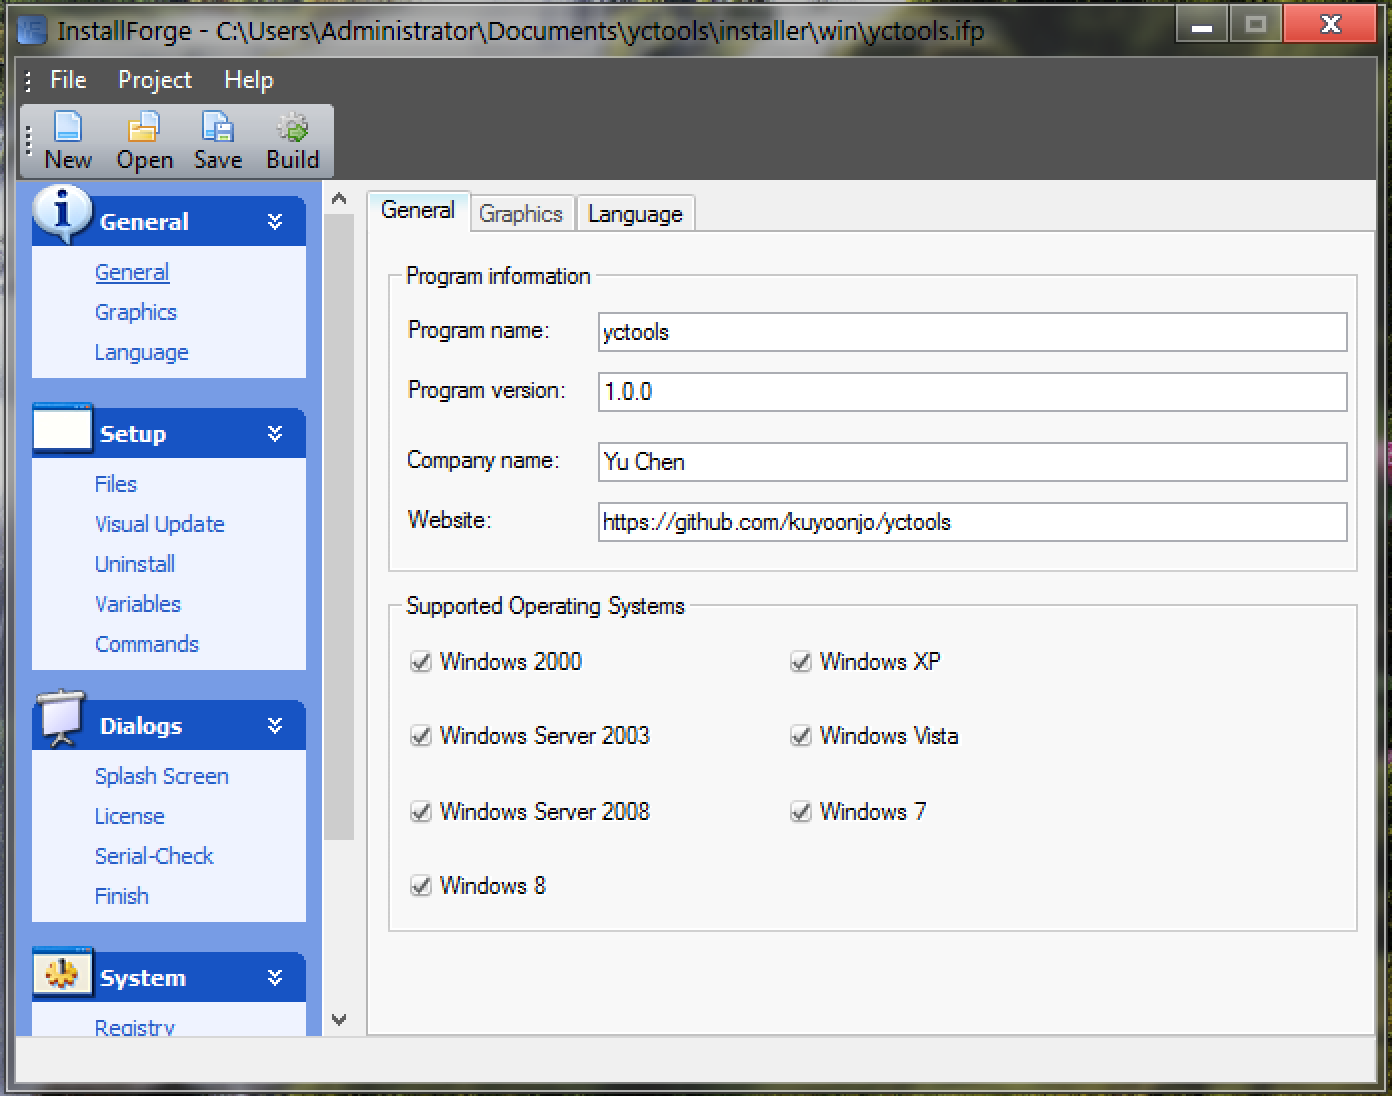
\includegraphics[width=\textwidth,height=\textheight/2,keepaspectratio=true]{ResearchInstallForge.png}}
\end{DoxyImageNoCaption}
\hypertarget{_software_packaging_SoftwarePackagingDebianPackageManagement}{}\section{Debian Package Management}\label{_software_packaging_SoftwarePackagingDebianPackageManagement}
Debian packages generally contain all of the files necessary to implement a set of related commands or features. ~\newline
~\newline
A Debian binary package can contain\+:
\begin{DoxyItemize}
\item executable files
\item configuration files
\item man pages
\item copyright information
\item relative documentation. Linux distributions use Debian package management\+:
\item Ubuntu
\item Debian
\end{DoxyItemize}

Debreate is a Debian package builder. It makes it easy to use graphical user interface for packaging applications. \cite{debreate} 
\begin{DoxyImageNoCaption}
  \mbox{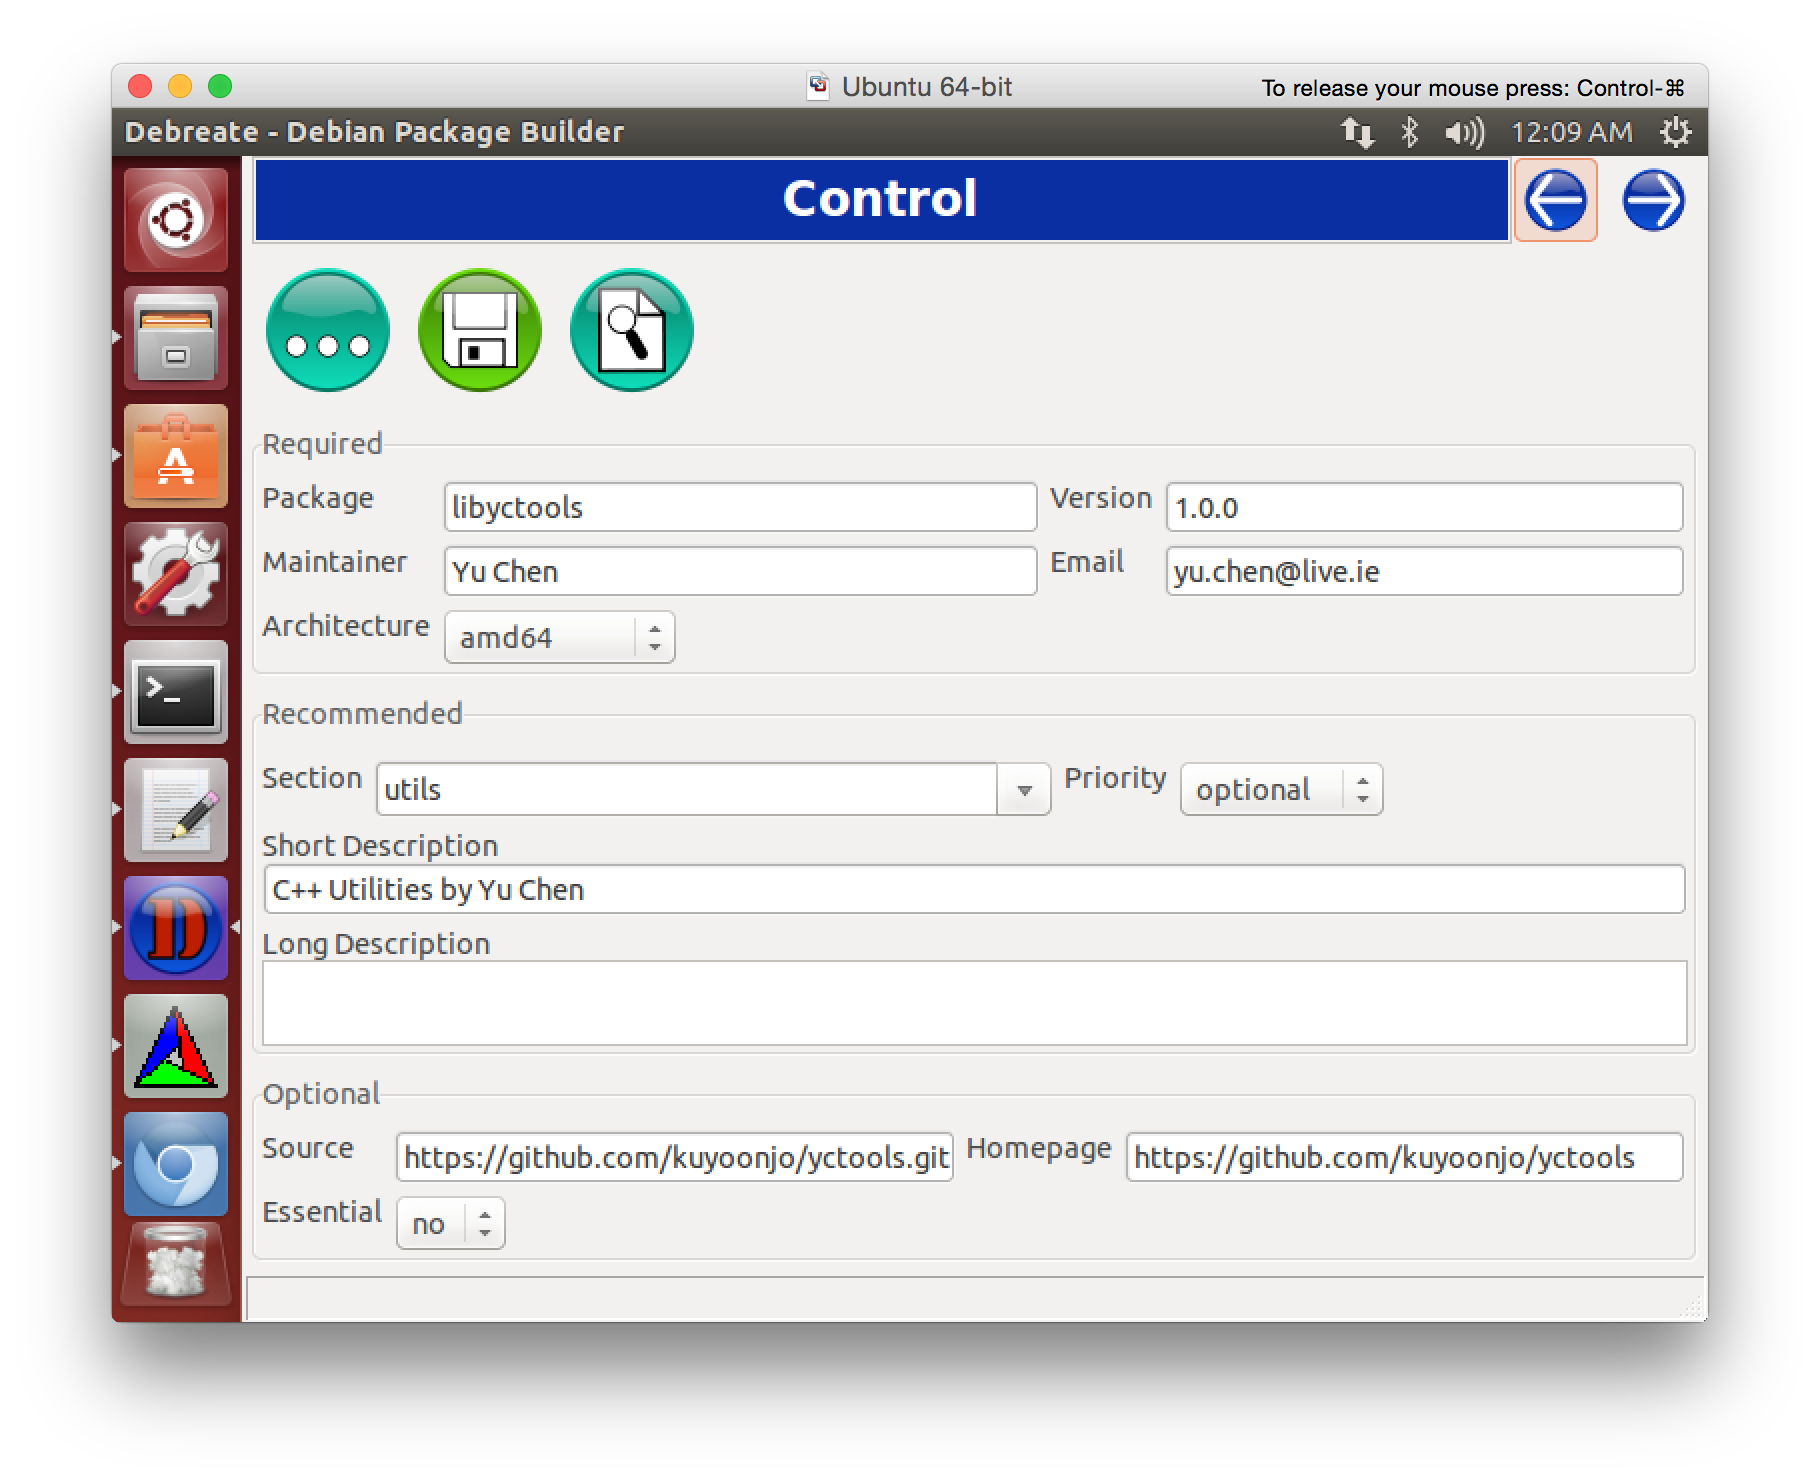
\includegraphics[width=\textwidth,height=\textheight/2,keepaspectratio=true]{ResearchDebreate.png}}
\end{DoxyImageNoCaption}
 
\chapter{Conclusion}
\label{_conclusion}
\hypertarget{_conclusion}{}
After looking into all of the differences, I have decided to use Intel T\+B\+B to develop the library. Open\+M\+P is easy to use however, it uses compiler directives, which means not all compiler support Open\+M\+P. For example, the default compiler in Mac O\+S X does not support Open\+M\+P. Intel T\+B\+B is a library developed by C++ so that any C++ compiler can use it. ~\newline
~\newline
Because Intel T\+B\+B is a C++ library, so the programming language is C++. The graphic library will be S\+F\+M\+L because of the object oriented programming. Also, S\+F\+M\+L is available in multiple platform. The C++ I\+D\+E is Xcode, which has the best performance under Mac system. It has a serious of tools for debugging such as memory leak detector. Also, use Xcode to create Mac application bundles will be very simple. However, this project is not only for Mac users, so I will use C\+Make to make the project portable for other operating systems. ~\newline
~\newline
I will use Git for source control because it is the most powerful and most widely used. Github provides a free service that user can create public repositories for free. Doxygen, Graphviz, and La\+Tex will be used for documentation. Doxygen can generate document from code. Graphviz can create class diagrams from code. The reason I choose La\+Tex indeed of visible document editors like Microsoft Word, Google Doc, or Apple Pages is that Doxygen can only generate html and latex documents. ~\newline
~\newline
Package\+Maker, Installforge, and Debreate will be used for Mac O\+S X, Microsoft Window, and Debian-\/like Linux. All of them are G\+U\+I and simple. 
%--- End generated contents ---

% Bibliography
\newpage
\phantomsection
\bibliographystyle{plain}
\bibliography{bibTmpFile_1}
\addcontentsline{toc}{chapter}{Bibliography}

% Index
\backmatter
\newpage
\phantomsection
\clearemptydoublepage
\addcontentsline{toc}{chapter}{Index}
\printindex

\end{document}
